\subsection{Opgave 13}

Figuren viser en trekant\\\\
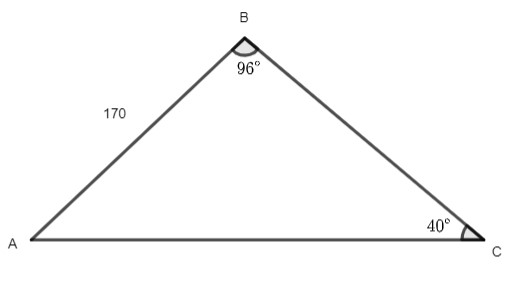
\includegraphics[width=10cm]{Opgave_11-20/Opgave_13/Opgave_13.jpg}\\\\
Følgende størrelser i trekant $ABC$ er kendte:\\\\
$B = 96^{\circ},\quad |AB| = 170\quad \text{og}\quad C = 40^{\circ}$\\\\

Bestem $|AC|$.\\\\

\ans
For at bestemme længden af siden $AC$ bruger vi sinusrelationen for en vilkårlig trekant
\begin{align*}
    \frac{a}{\sin(A)} = \frac{b}{\sin(B)} = \frac{c}{\sin(C)}
\end{align*}
Her svarer sidelængen $AB$ til c og sidelængden $AC$ som vi skal finde svarer til b. Vi betragter den sidste lighed i sinusrelationen og isolerer b.
\begin{align*}
    \frac{b}{\sin(B)} =\frac{c}{\sin(C)} \Longleftrightarrow b = \frac{c}{\sin(C)}\cdot \sin(B)
\end{align*}
Indsætter nu $c = 170,\quad C = 40^{\circ},\quad B = 96^{\circ}$ og får 
\begin{align*}
    b = \frac{170}{\sin(40^{\circ})}\cdot \sin(96^{\circ})\approx 263.03
\end{align*}